\section{Einleitung}
Hallo!
Du willst mit dem NAO-Roboter arbeiten? Kann ich nachvollziehen, er ist ziemlich süß. Doch wie fängt man an? Lass es und zusammen herausfinden!

\section{Set-Up}
\subsection{Choreograph}
\begin{itemize}
    \item Melde dich auf dem Windows PC an
    \item Öffne Choreograph auf dem Windows-PC
    \item Erstelle ein neues Projekt, oder öffne ein bestehendes
    \item Gehe in die Benutzereinstellungen und stelle die Sprache auf deutsch %TODO%
\end{itemize}

\subsection{Verbinde dich mit dem NAO}
Um zu gucken, ob dein Programm, welches du geschrieben hast auch wirklich läuft. Solltest du es am besten direkt mit dem NAO testen. Dazu musst du dich mit ihm verbinden. Doch wie geht das?
\subsubsection{Verbinde dich über das WIFI}
Du kannst NAO entweder über eine kabelgebundene oder eine WiFi-Verbindung mit deinem Computer verbinden:

\begin{enumerate}
    \item Entferne die Abdeckung hinter dem Kopf des Roboters, um Zugang zur Ethernet-Buchse zu erhalten.
    \item Schließe ein Ethernet-Kabel an.
    \begin{figure}[h]
        \centering
        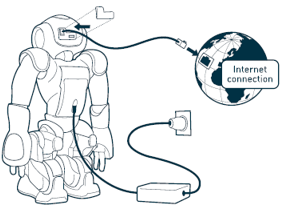
\includegraphics[width=0.2\textwidth]{../images/pluginEthernatCabel.png}
        \label{fig:pluginEthernatCabel}
    \end{figure}
    \item Verbinde das Ethernet-Kabel mit deinem Internet-Router. Weitere Details findest du unter: \href{https://doc.aldebaran.com/2-1/nao/nao-connecting.html}{Anschließen meines Roboters an Ethernet}.
    \item Greife auf die NAO-Webseite zu und melde dich an. Weitere Details findest du unter: \href{https://doc.aldebaran.com/2-1/nao/nao-connecting.html}{Zugriff auf die NAO-Webseite}.
    \item Wähle und konfiguriere im Bereich "Netzwerkeinstellungen" ein WiFi-Netzwerk.
\end{enumerate}
\textbf{Ergebnis:} Die WiFi-Verbindung ist eingerichtet. Du kannst nun das Ethernet-Kabel entfernen und die Abdeckung hinter dem Kopf des Roboters schließen.

\subsubsection{Einrichten der kabelgebundenen Verbindung}
\textbf{Achtung:} Stelle sicher, dass NAO nicht mit einem Ethernet-Kabel verbunden ist, während er sich bewegt, da das Kabel gezogen werden und der Anschluss beschädigt werden könnte.
\begin{enumerate}
    \item Entferne die Abdeckung hinter dem Kopf des Roboters, um Zugang zur Ethernet-Buchse zu erhalten.
    \item Schließe ein Ethernet-Kabel an.
    \item Verbinde das Ethernet-Kabel mit deinem Internet-Router. Weitere Details findest du unter: \href{https://doc.aldebaran.com/2-1/nao/nao-connecting.html}{Anschließen meines Roboters an Ethernet}.
    \item Das kabelgebundene Netzwerk erscheint in der Liste.
    \item Wähle das kabelgebundene Netzwerk aus.
\end{enumerate}
\subsubsection{Virtueller Roboter Emulator}
Der virtuelle Roboter Emulator in Choregraphe ermöglicht dir, den NAO-Roboter in einer simulierten Umgebung zu steuern, bevor du Aktionen auf einem physischen Roboter ausführst. Dies ist besonders nützlich, um Prototypen zu erstellen und komplexe Bewegungen zu testen. Der Emulator zeigt den NAO in einer 3D-Ansicht und ermöglicht es dir, Aktionen wie Bewegungen, Interaktionen und sensorische Inputs zu testen. Die Integration in Choregraphe bietet eine nahtlose Möglichkeit, Skripte auszuführen und schnell Feedback zu erhalten, bevor du sie auf dem realen Roboter ausführst.
Um den virtuellen Roboter Emulator in Choregraphe zu nutzen, folge diesen Schritten:
\begin{enumerate}
    \item \textbf{Verbindung zum virtuellen Roboter herstellen}: Klicke auf das Symbol \texttt{Verbindung} und wähle die Option \texttt{Virtueller Roboter}. Dadurch wird eine simulierte Version des NAO gestartet.
    \item \textbf{Erstellen und Testen von Abläufen}: Du kannst durch Drag-and-Drop von Boxen im \texttt{Diagramm-Editor} Bewegungsabläufe und Interaktionen erstellen.
    \item \textbf{Skripte und Aktionen ausführen}: Klicke auf \texttt{Play}, um dein Skript im Emulator auszuführen. Der virtuelle NAO wird deine Aktionen simulieren, und du kannst seine Bewegungen und Interaktionen in Echtzeit beobachten.
\end{enumerate}
Durch den Emulator kannst du sicherstellen, dass deine Programme effizient arbeiten und korrekt ablaufen, ohne direkt auf einem echten Roboter zu testen, was Zeit und mögliche Risiken spart.

Weiter Möglichkeiten dich mit NAO zu verbinden findest du hier: \href{http://doc.aldebaran.com/2-8/family/nao_user_guide/nao-connecting.html}. 

\section{Debugging mit Log-Funktionen}
Das Debugging mit Log-Funktionen ist eine wichtige Methode, um Probleme im Code zu identifizieren und das Verhalten des NAO-Roboters während der Ausführung von Programmen zu analysieren. Choregraphe bietet eine integrierte \texttt{Log Viewer}-Funktion, die du nutzen kannst, um detaillierte Informationen zur Programmausführung zu erhalten. Durch das Einfügen von \texttt{print}-Anweisungen oder speziellen Log-Methoden in den Code kannst du den Status und die Ergebnisse von Operationen während der Laufzeit einsehen.

\subsection{Verwendung der Log Viewer-Funktion}
Um den Log Viewer effektiv zu nutzen, folge diesen Schritten:
\begin{enumerate}
    \item \textbf{Öffnen des Log Viewers}: Klicke auf \texttt{Ansicht} in der Menüleiste und wähle \texttt{Log Viewer}, um das Log-Fenster zu öffnen. Hier werden alle Log-Meldungen in Echtzeit während der Programmausführung angezeigt.
    \item \textbf{Hinzufügen von Log-Nachrichten im Code}: Füge \texttt{print}-Anweisungen in deinem Python-Code ein, um spezifische Informationen während der Ausführung auszugeben. Diese Nachrichten erscheinen im Log Viewer und helfen dir, den Ablauf des Programms zu verstehen.
    \item \textbf{Starten der Programmausführung}: Klicke auf \texttt{Play}, um das Programm im \texttt{Diagramm-Editor} auszuführen. Der Log Viewer zeigt dann alle Ausgaben an, die im Code durch \texttt{print} oder spezielle Debugging-Methoden erzeugt wurden.
    \item \textbf{Überprüfen der Ausgaben}: Während das Programm läuft, kannst du die Nachrichten im Log Viewer beobachten, um sicherzustellen, dass alle Aktionen wie erwartet ablaufen. Falls Fehler oder unerwartete Werte auftreten, kannst du diese hier sofort sehen.
\end{enumerate}

\subsection{Hinzufügen von Log-Nachrichten im Code}
Um gezielte Informationen aus deinem Code im Log Viewer anzuzeigen, kannst du verschiedene Techniken nutzen:
\begin{itemize}
    \item \textbf{Print-Anweisungen}: Die einfachste Methode ist die Verwendung von \texttt{print("Nachricht")} im Code. Dies ist besonders nützlich, um Variablenwerte und den Ablauf der Programmschritte anzuzeigen.
    \item \textbf{ALLogger API}: Für umfangreiches Logging kannst du die \texttt{ALLogger}-API verwenden, die spezifische Meldungen für verschiedene Log-Level (z.B. \texttt{INFO}, \texttt{WARNING}, \texttt{ERROR}) unterstützt. Beispiel:
    \begin{verbatim}
    self.logger = ALProxy("ALLogger")
    self.logger.info("MyBox", "Dies ist eine Info-Nachricht.")
    self.logger.warning("MyBox", "Dies ist eine Warnung.")
    self.logger.error("MyBox", "Dies ist eine Fehlermeldung.")
    \end{verbatim}
    \item \textbf{Fehlersuche bei Eingabe- und Ausgabe-Ereignissen}: Verwende Log-Nachrichten, um den Empfang und die Verarbeitung von Events und Eingaben zu verfolgen. Füge z.B. eine \texttt{print}-Anweisung am Anfang einer \texttt{onInput\_x} Methode ein, um zu bestätigen, dass die Methode aufgerufen wird.
\end{itemize}

\subsection{Interpretation der Log-Nachrichten}
Nachdem du das Programm ausgeführt hast und Log-Nachrichten im Log Viewer erscheinen, solltest du Folgendes beachten:
\begin{itemize}
    \item \textbf{Abfolge der Meldungen}: Die Reihenfolge der Nachrichten hilft dir zu verstehen, ob die Programmschritte in der gewünschten Reihenfolge ausgeführt werden.
    \item \textbf{Fehlermeldungen}: Falls Fehler auftreten, analysiere die Fehlermeldungen. Der Log Viewer zeigt oft den genauen Ort im Code und eine Beschreibung des Fehlers an.
    \item \textbf{Variablen und Zustände prüfen}: Durch Ausgaben von Variablenwerten und Zuständen kannst du feststellen, ob bestimmte Werte oder Abläufe korrekt verarbeitet werden.
\end{itemize}

\subsection{Beispiel für das Debugging mit Log-Nachrichten}
Hier ist ein Beispiel, wie du Log-Nachrichten in einer benutzerdefinierten Box verwenden kannst:
\begin{verbatim}
class MyCustomBoxClass(ALModule):
    def onInput_onStart(self):
        print("Start-Input empfangen.")
        self.logger.info("MyBox", "Der Start-Input wurde erfolgreich empfangen.")
        
        # Beispielhafte Berechnung
        result = 10 * 2
        print("Ergebnis der Berechnung:", result)
        self.logger.info("MyBox", "Ergebnis der Berechnung: " + str(result))
\end{verbatim}
In diesem Beispiel wird sowohl mit \texttt{print} als auch mit der \texttt{ALLogger}-API der Ablauf der Programmschritte protokolliert. Dies erleichtert die Fehlersuche und gibt dir einen genauen Überblick über die Ausführung.

\section{Events}\label{events}
Events sind ein zentraler Bestandteil in Choregraphe, um Aktionen und Reaktionen des NAO-Roboters zu steuern. Sie ermöglichen es, dynamische und interaktive Abläufe zu erstellen, die auf spezifische Ereignisse reagieren. Events können durch Benutzereingaben, Sensorwerte, Zeitabläufe oder andere Zustände ausgelöst werden und steuern das Verhalten der Boxen in einem Projekt.
\begin{figure}[h]
    \centering
    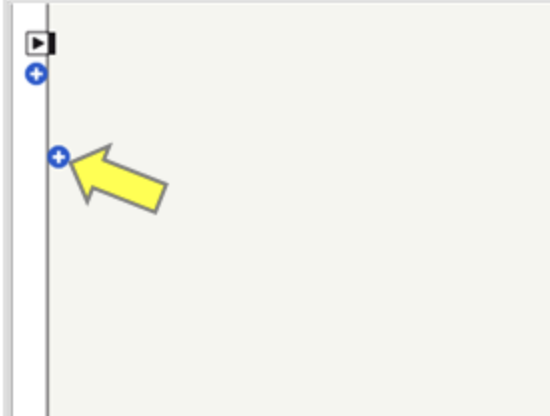
\includegraphics[width=0.1\textwidth]{../images/event.png}
    \label{fig:event}
\end{figure}
\subsection{Definition und Bedeutung von Events}
Ein Event ist eine Benachrichtigung oder ein Signal, das anzeigt, dass ein bestimmter Zustand oder ein bestimmtes Ereignis eingetreten ist. Sobald ein Event ausgelöst wird, können andere Boxen, die auf dieses Event hören, eine definierte Aktion ausführen. Events ermöglichen die Kommunikation zwischen verschiedenen Boxen und sind essenziell, um komplexe, ereignisgesteuerte Programme zu erstellen.

\subsection{Arten von Events}
In Choregraphe gibt es verschiedene Arten von Events, die unterschiedliche Zwecke erfüllen:
\begin{itemize}
    \item \textbf{System-Events}: Diese Events werden durch das System oder den NAO-Roboter selbst generiert, z.B. das Erreichen eines Bewegungsziels oder das Erkennen einer Berührung.
    \item \textbf{Benutzerdefinierte Events}: Du kannst benutzerdefinierte Events erstellen, die speziell für die Anforderungen deines Programms entwickelt werden. Diese können durch benutzerdefinierten Code ausgelöst und mit anderen Boxen verknüpft werden.
    \item \textbf{Sensor-Events}: Diese Events werden ausgelöst, wenn ein bestimmter Zustand eines Sensors erkannt wird, z.B. Berührungen an einem bestimmten Punkt des Roboters oder die Erkennung von Gesichtern.
    \item \textbf{Timer-Events}: Timer-Events basieren auf zeitlichen Abläufen und werden nach Ablauf eines definierten Zeitraums oder in festgelegten Intervallen ausgelöst.
\end{itemize}

\subsection{Erstellen und Konfigurieren von Events}
Um ein Event in Choregraphe zu erstellen oder zu konfigurieren, kannst du die folgenden Schritte ausführen:
\begin{enumerate}
    \item \textbf{Verbindung zwischen Boxen herstellen}: Um ein Event auszulösen, verbinde den Output einer Box, die das Event auslöst, mit dem Input einer anderen Box, die auf das Event reagieren soll.
    \item \textbf{Benutzerdefinierte Events definieren}: Falls du ein benutzerdefiniertes Event benötigst, kannst du es in deinem Python-Code innerhalb der Box definieren und mit der \texttt{raiseEvent}-Funktion auslösen.
    \begin{verbatim}
    self.raiseEvent("MyCustomEvent", "Eventwert")
    \end{verbatim}
    \item \textbf{Reaktionslogik festlegen}: Verwende die Eigenschaften der Zielbox, um die gewünschte Reaktion auf das Event zu definieren. Dies könnte das Starten einer Bewegung, das Abspielen eines Sounds oder eine beliebige andere Aktion sein.
    \item \textbf{Ereignisbedingungen setzen}: Falls erforderlich, kannst du Bedingungen für die Auslösung eines Events festlegen. Dies ermöglicht dir, komplexe Regeln und Interaktionsmuster zu erstellen.
\end{enumerate}

\subsection{Verknüpfung und Nutzung von Events}
Events können auf verschiedene Weise genutzt und verknüpft werden:
\begin{itemize}
    \item \textbf{Kaskadierende Events}: Ein Event kann mehrere andere Events auslösen, indem es mit mehreren Inputs verschiedener Boxen verbunden ist. Dies ist besonders nützlich für komplexe Interaktionen, bei denen mehrere Aktionen als Reaktion auf ein einzelnes Event stattfinden sollen.
    \item \textbf{Priorisierung von Events}: Falls mehrere Events gleichzeitig ausgelöst werden, kannst du die Priorität und die Reihenfolge der Verarbeitung festlegen, um sicherzustellen, dass kritische Aktionen zuerst ausgeführt werden.
    \item \textbf{Event-Listener}: Eine Box kann als \texttt{Listener} für ein bestimmtes Event fungieren und so auf jede Auslösung des Events reagieren. Dies ermöglicht ereignisgesteuerte Logik und erhöht die Flexibilität des Programms.
\end{itemize}

\subsection{Beispiele für die Verwendung von Events}
Hier sind einige typische Anwendungsfälle für Events:
\begin{itemize}
    \item \textbf{Reaktion auf Berührung}: Ein \texttt{Sensor-Event} wird ausgelöst, wenn der Kopf des NAO berührt wird, und eine verbundene Box startet eine Sprachansage.
    \item \textbf{Zeitschleifen}: Ein \texttt{Timer-Event} löst regelmäßig eine bestimmte Bewegung aus, wodurch eine Wiederholungsschleife entsteht.
    \item \textbf{Benutzerinteraktion}: Ein \texttt{Benutzerdefiniertes Event} wird ausgelöst, wenn ein spezifisches Sprachkommando erkannt wird, was eine Reaktion wie eine Begrüßung oder eine Animation startet.
\end{itemize}

Durch die Nutzung und das Verständnis von Events kannst du das Verhalten des NAO-Roboters flexibel und komplex gestalten und auf externe Ereignisse und Benutzerinteraktionen reagieren.

\section{Inputs und Outputs in Events und Boxen}
In Choregraphe kannst du die Logik des NAO-Roboters durch sogenannte Boxen (Blöcke) darstellen. Jede Box kann verschiedene Inputs (Eingaben) und Outputs (Ausgaben) haben, die du für Events und Aktionen verwenden kannst:
\begin{itemize}
    \item \textbf{Inputs}: Steuern, wie eine Box auf externe Ereignisse reagiert. Sie sind die Eingänge, die du mit anderen Boxen verbinden kannst.
    \item \textbf{Outputs}: Sind die Ausgaben, die von einer Box generiert werden und können mit anderen Boxen verbunden werden, um komplexere Logik und Handlungen auszulösen.
\end{itemize}

\subsection{Eigenschaften von Inputs}
Inputs bestimmen, wie eine Box auf externe Ereignisse reagiert. Die wichtigsten Eigenschaften von Inputs umfassen:
\begin{itemize}
    \item \textbf{Name des Inputs}: Der Name dient zur Identifizierung des Inputs und wird im Diagramm-Editor angezeigt. Es ist wichtig, einen aussagekräftigen Namen zu wählen, der den Zweck des Inputs beschreibt.
    \item \textbf{Typ des Inputs}: Der Typ definiert, welche Art von Daten der Input akzeptiert. Dies können einfache Datentypen (wie \texttt{int}, \texttt{float} oder \texttt{string}) oder komplexere Objekte sein. Der Typ sollte den Anforderungen der Logik in der Box entsprechen.
    \item \textbf{Beschreibung}: Ein optionales Textfeld, das die Funktion des Inputs erläutert. Die Beschreibung hilft anderen Nutzern oder dir selbst dabei, den Zweck und die Funktionsweise des Inputs schnell zu verstehen.
    \item \textbf{Eingangsbedingungen}: Du kannst Bedingungen festlegen, unter denen der Input aktiviert oder ausgelöst wird \ref{events}. Dies ermöglicht eine präzisere Steuerung der Box-Logik und verhindert ungewollte Aktionen.
    \item \textbf{Verbindungen}: Jeder Input kann mit einem oder mehreren Outputs anderer Boxen verbunden werden. Durch das Verbinden werden die Events und Daten zwischen verschiedenen Boxen weitergeleitet und verarbeitet.
\end{itemize}

\subsection{Eigenschaften von Outputs}
Outputs bestimmen, welche Ereignisse oder Daten von einer Box ausgegeben werden. Die wichtigsten Eigenschaften von Outputs umfassen:
\begin{itemize}
    \item \textbf{Name des Outputs}: Der Name dient zur Identifikation des Outputs und sollte klar und präzise benennen, welche Art von Daten oder Ereignissen ausgegeben wird.
    \item \textbf{Typ des Outputs}: Ähnlich wie bei Inputs definiert der Typ des Outputs, welche Art von Daten ausgegeben wird. Dies kann beispielsweise ein einfacher Datentyp wie \texttt{boolean} oder ein komplexes Objekt sein.
    \item \textbf{Beschreibung}: Eine optionale Beschreibung des Outputs, die erklärt, welche Daten oder Ereignisse ausgegeben werden. Dies ist nützlich, um die Logik der Box für andere Nutzer verständlich zu machen.
    \item \textbf{Auslösebedingungen}: Du kannst angeben, unter welchen Bedingungen der Output ausgelöst wird \ref{events}. Dies kann durch bestimmte Ereignisse oder durch das Erfüllen von Bedingungen innerhalb der Box geschehen.
    \item \textbf{Verbindungen zu anderen Boxen}: Ein Output kann mit einem oder mehreren Inputs anderer Boxen verbunden werden. Dies ermöglicht es, Ereignisse oder Daten weiterzugeben und so komplexere Interaktionen und Abläufe zu gestalten.
\end{itemize}

\subsection{Parameter von Inputs und Outputs}
Inputs und Outputs können mit verschiedenen Parametern ausgestattet sein, die deren Verhalten steuern:
\begin{itemize}
    \item \textbf{Standardwert}: Für Inputs kann ein Standardwert festgelegt werden, der verwendet wird, falls keine externe Eingabe erfolgt. Dies stellt sicher, dass die Box einen definierten Zustand hat, auch wenn kein externes Signal vorliegt.
    \item \textbf{Datenformat}: Es kann angegeben werden, in welchem Format Daten akzeptiert oder ausgegeben werden. Zum Beispiel können numerische Werte als \texttt{int} oder \texttt{float} und Texte als \texttt{string} definiert werden.
    \item \textbf{Trigger-Typ}: Für Outputs kannst du festlegen, ob der Output nur einmalig ausgelöst wird oder ob er kontinuierlich Werte sendet, solange bestimmte Bedingungen erfüllt sind \ref{events}.
    \item \textbf{Verarbeitungsreihenfolge}: Die Reihenfolge, in der Inputs verarbeitet werden, kann konfiguriert werden. Dies ist nützlich, wenn mehrere Inputs gleichzeitig eintreffen und priorisiert verarbeitet werden müssen.
    \item \textbf{Verbindungstyp}: Inputs und Outputs können auf verschiedene Weise mit anderen Boxen verbunden werden. Du kannst einstellen, ob die Verbindung direkt (Synchronisation der Daten) oder ereignisbasiert erfolgt (nur bei bestimmten Ereignissen).
\end{itemize}

Die detaillierte Konfiguration von Inputs und Outputs ermöglicht dir eine präzise Steuerung der Logik innerhalb deines Programms und erlaubt es, komplexe Interaktionen zwischen den verschiedenen Boxen in Choregraphe zu gestalten.
\subsection{Hinzufügen neuer Inputs und Outputs}
Um neue Inputs oder Outputs zu einer Box hinzuzufügen, kannst du folgende Schritte ausführen:
\begin{enumerate}
    \item \textbf{Box auswählen}: Klicke im \texttt{Diagramm-Editor} auf die Box, die du konfigurieren möchtest.
    \item \textbf{Eigenschaften öffnen}: Gehe zu den \texttt{Eigenschaften} der Box, indem du sie doppelklickst oder mit der rechten Maustaste darauf klickst und \texttt{Eigenschaften anzeigen} auswählst.
    \item \textbf{Neuen Input/Output hinzufügen}: Nutze die \texttt{Input/Output}-Registerkarte und wähle \texttt{Neuer Input hinzufügen} oder \texttt{Neuer Output hinzufügen}. Du kannst die Typen, Namen und Beschreibungen entsprechend festlegen.
    \item \textbf{Verbindungen herstellen}: Ziehe Verbindungen von den neuen Inputs oder Outputs zu anderen Boxen, um deine gewünschte Logik zu erstellen.
\end{enumerate}

\subsection{Konfigurieren bestehender Inputs und Outputs}
Die Konfiguration bestehender Inputs und Outputs ermöglicht es dir, deren Verhalten anzupassen:
\begin{enumerate}
    \item \textbf{Eigenschaften öffnen}: Öffne die Box, indem du sie doppelklickst oder \texttt{Eigenschaften} über das Kontextmenü wählst.
    \item \textbf{Parameter ändern}: Du kannst Namen, Beschreibungen oder Verbindungen der Inputs und Outputs ändern. Gehe zu den entsprechenden \texttt{Input/Output}-Einstellungen und passe die Parameter nach Bedarf an.
    \item \textbf{Bedingungen und Filter}: Falls gewünscht, kannst du spezielle Bedingungen oder Filter auf die Inputs und Outputs anwenden, um deren Verhalten weiter zu spezifizieren.
\end{enumerate}

\subsection{Löschen von Inputs und Outputs}
Wenn du Inputs oder Outputs nicht mehr benötigst, kannst du sie einfach entfernen:
\begin{enumerate}
    \item \textbf{Box auswählen}: Markiere die Box, aus der du Inputs oder Outputs löschen möchtest.
    \item \textbf{Input/Output-Einstellungen aufrufen}: Gehe zu den \texttt{Input/Output}-Registerkarten in den Box-Eigenschaften.
    \item \textbf{Auswahl löschen}: Wähle den Input oder Output, den du löschen möchtest, und klicke auf \texttt{Entfernen} oder nutze die entsprechende Schaltfläche.
    \item \textbf{Verbindungen prüfen}: Nach dem Löschen solltest du sicherstellen, dass keine ungenutzten Verbindungen übrig bleiben, die Probleme verursachen könnten.
\end{enumerate}

\section{Standartboxen}
Hier sind die Boxen, die standardmäßig in Choregraphe enthalten sind und die du somit direkt benutzen kannst, und deren Funktionen:
\begin{itemize}
    \item \textbf{Behavior Box}: Diese Box steuert das Verhalten des NAO-Roboters in einer bestimmten Situation. Sie kann komplexe Abfolgen von Bewegungen, Audio- und Sensoreingaben kapseln, um zusammenhängende Aktionen auszuführen. Die Behavior Box kann auch verschachtelte Abläufe und Verzweigungen enthalten.
    \item \textbf{Sound Box}: Mit dieser Box kann der NAO Klänge abspielen oder Texte vorlesen. Du kannst vordefinierte Audiodateien abspielen oder NAO mit der Text-zu-Sprache-Funktion Inhalte sprechen lassen. Die Sound Box kann auch an verschiedene Triggerpunkte gebunden werden, um reaktive Kommunikation zu ermöglichen.
    \item \textbf{Movement Box}: Diese Box steuert die Bewegungen des Körpers, der Arme, des Kopfes und anderer beweglicher Teile des NAO. Du kannst Bewegungsabläufe entweder vorgefertigt abspielen oder über die \texttt{Timeline}-Ansicht detailliert anpassen. Hier lassen sich auch Übergänge und Synchronisation mit anderen Aktionen einfügen.
    \item \textbf{Wait Box}: Die Wait Box ermöglicht es dir, den Roboter für eine bestimmte Zeit warten zu lassen, bevor die nächste Aktion ausgeführt wird. Dies kann nützlich sein, um zeitlich abgestimmte Bewegungen oder Interaktionen zu planen. Die Dauer kann in Sekunden oder anderen Einheiten angegeben werden. Es gibt die Wait time (zeit abwarten) box und die Wait-for (auf etwas bestimmtes warten).
    \begin{figure}[h]
        \centering
        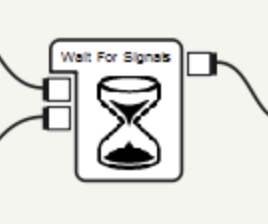
\includegraphics[width=0.1\textwidth]{../images/waitBox.png}
        \label{fig:waitBox}
    \end{figure}
    \item \textbf{Sensor Box}: Diese Box nutzt eingehende Sensordaten (z.B. Berührungen, Infrarot, Kameradaten) und reagiert entsprechend. Du kannst Regeln und Bedingungen erstellen, die auf den Sensoreingaben basieren und eine Aktion auslösen.
    \item \textbf{LED Box}: Mit dieser Box kannst du die LEDs am NAO-Roboter steuern. Du kannst Muster, Farben und Helligkeit verändern, um Stimmungen, Statusanzeigen oder Signale zu kommunizieren. Die LED Box ist besonders nützlich, um visuelles Feedback zu geben oder auf bestimmte Ereignisse zu reagieren.
    \item \textbf{Speech Recognition Box}: Diese Box ermöglicht es dem NAO, Sprachbefehle zu erkennen und darauf zu reagieren. Du kannst eine Liste von Schlüsselwörtern definieren, auf die der Roboter hören soll, und entsprechende Aktionen mit diesen Ereignissen verknüpfen.
    \item \textbf{Animation Box}: Die Animation Box enthält vorgefertigte Bewegungssequenzen, die aus dem Standardanimationskatalog des NAO geladen werden können. Diese sind besonders nützlich, um realistische Bewegungen oder vordefinierte Verhaltensweisen zu verwenden, ohne sie von Grund auf neu erstellen zu müssen.
    \begin{figure}[h]
        \centering
        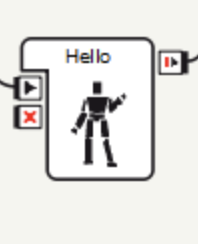
\includegraphics[width=0.1\textwidth]{../images/animationBox.png}
        \label{fig:animationBox}
    \end{figure} 
    \item \textbf{Face Detection Box}: Diese Box ermöglicht es dem NAO, Gesichter zu erkennen und zu verfolgen. Sie kann mit Aktionen verknüpft werden, die auf das Erkennen oder Verfolgen von Gesichtern reagieren, z.B. das Sprechen mit einer Person oder das Drehen des Kopfes.
    \item \textbf{Video Box}: Die Video Box bietet Zugriff auf die Kameras des NAO-Roboters. Du kannst Videostreams verwenden, um Bilder zu erfassen, Videosequenzen aufzuzeichnen oder visuelle Analysen durchzuführen, wie z.B. die Erkennung von Mustern oder Objekten.
    \item \textbf{Dialog Box}: Diese Box erlaubt die Verwaltung von Dialogen mit dem NAO. Du kannst komplexe Gesprächslogiken erstellen und NAO auf spezifische Wörter oder Phrasen reagieren lassen, wodurch eine interaktive Kommunikation mit Menschen möglich wird.
    \item \textbf{Loop Box}: Mit der Loop Box kannst du Schleifen implementieren, sodass eine Aktion oder ein Verhalten wiederholt ausgeführt wird. Dies ist besonders nützlich für iterative Prozesse oder zeitlich wiederkehrende Aufgaben.
    \item \textbf{For Box}: Mit der For Box kannst du Schleifen implementieren, sodass eine Aktion oder ein Verhalten wiederholt ausgeführt wird. Dies ist besonders nützlich für iterative Prozesse oder zeitlich wiederkehrende Aufgaben.
    \begin{figure}[h]
        \centering
        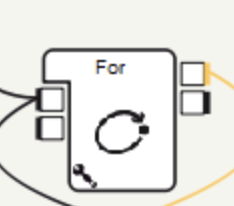
\includegraphics[width=0.1\textwidth]{../images/forBox.png}
        \label{fig:forBox}
    \end{figure}
    \item \textbf{Timer Box}: Diese Box startet einen Timer und löst nach Ablauf eine Aktion aus. Sie ist besonders nützlich, wenn du bestimmte Zeitabläufe in deinem Programmablauf steuern möchtest.
    \begin{figure}[h]
        \centering
        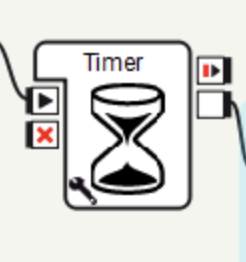
\includegraphics[width=0.1\textwidth]{../images/timerBox.png}
        \label{fig:timerBox}
    \end{figure} 
    \item \textbf{If Box}: Die Conditional Box erlaubt es, bedingte Logik zu implementieren. Basierend auf einem bestimmten Zustand oder einer Bedingung kannst du entscheiden, welcher Pfad in deinem Programmablauf ausgeführt wird. Dies ist nützlich, um die Entscheidungen des Roboters dynamisch zu steuern.
    \begin{figure}[h]
        \centering
        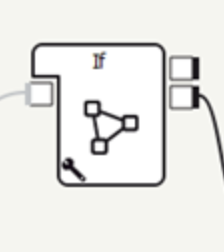
\includegraphics[width=0.1\textwidth]{../images/ifBox.png}
        \label{fig:ifBox}
    \end{figure} 
    \item \textbf{ALMemory Access Box}: Diese Box ermöglicht den Zugriff auf den Speicher des NAO-Roboters (\texttt{ALMemory}). Du kannst Daten lesen oder schreiben und so wichtige Zustandsinformationen austauschen oder Events überwachen.
    \item \textbf{Switch Case Box}: Diese Box ermöglicht es dir, verschiedene Pfade im Programmablauf abhängig vom eingehenden Wert auszuwählen. Dies ist nützlich, um komplexere Entscheidungsbäume und Programmflüsse zu implementieren.
    \item \textbf{Image Display Box}: Mit dieser Box kannst du Bilder auf dem Bildschirm des NAO anzeigen (falls vorhanden). Dies kann nützlich sein, um visuelle Rückmeldungen zu geben oder mit Benutzern zu interagieren.
    \item \textbf{Random Box}: Diese Box ermöglicht das Erzeugen und Verwenden von Zufallswerten oder das zufällige Auswählen von Verhaltensweisen. Dies verleiht dem Verhalten des Roboters eine gewisse Unvorhersehbarkeit und Dynamik.
    \item \textbf{Posture Box}: Die Posture Box erlaubt es, den Roboter in vordefinierte Haltungen und Positionen zu bringen, z.B. Sitzen, Stehen oder Liegen. Dies ist hilfreich für sicheres Starten oder Beenden von Bewegungen.
    \item \textbf{Play Sound Box}: Die Play Sound Box ermöglicht es dem NAO-Roboter, vordefinierte oder benutzerdefinierte Audiodateien abzuspielen. Du kannst diese Box nutzen, um Geräusche, Musik, Töne oder andere Audiodateien auszugeben, die auf dem Roboter gespeichert sind. Die Wiedergabeoptionen können angepasst werden, um die Lautstärke, Wiederholungen oder das Verhalten nach dem Ende des Sounds zu steuern. Diese Box ist besonders nützlich, um akustisches Feedback zu geben, eine Interaktion zu unterstreichen oder Benutzer auf bestimmte Aktionen aufmerksam zu machen.
    \begin{figure}[h]
        \centering
        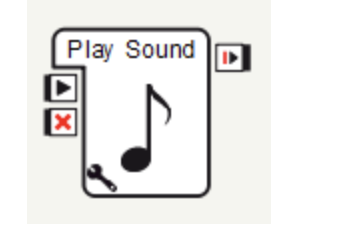
\includegraphics[width=0.1\textwidth]{../images/playSoundBox.png}
        \label{fig:playSoundBox}
    \end{figure}
    \item \textbf{Get File Path Box}: Die Get File Path Box ermöglicht es, den Pfad zu einer Datei im Dateisystem des NAO-Roboters oder auf einem verbundenen Computer abzurufen. Diese Box wird häufig verwendet, um Pfade zu Dateien wie Bildern, Audiodateien oder Skripten zu ermitteln, die später in anderen Boxen oder Prozessen verwendet werden können. Durch das Abrufen des Dateipfads kannst du flexibel mit Dateien arbeiten, die dynamisch ausgewählt oder in anderen Kontexten benötigt werden.
    \begin{figure}[h]
        \centering
        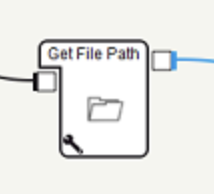
\includegraphics[width=0.1\textwidth]{../images/getFilePathBox.png}
        \label{fig:getFilePathBox}
    \end{figure}
    \item \textbf{Say Box}: Die Say Box ermöglicht es dem NAO-Roboter, Text laut auszusprechen, indem er die integrierte Text-zu-Sprache-Funktion (Text-to-Speech, TTS) verwendet. Du kannst diese Box nutzen, um dynamische Ansagen, vordefinierte Texte oder interaktive Antworten zu generieren. Die \texttt{Say Box} bietet eine einfache Möglichkeit, den NAO mit Menschen interagieren zu lassen und Sprachfeedback in Echtzeit zu geben.
    \begin{figure}[h]
        \centering
        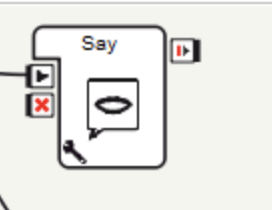
\includegraphics[width=0.1\textwidth]{../images/sayBox.png}
        \label{fig:sayBox}
    \end{figure}
\end{itemize}
\subsection{Zusammenfassung mehrerer Boxen in eine einzige Box}
Das Gruppieren mehrerer Boxen in eine einzige \texttt{Behavior Box} oder eine benutzerdefinierte Box bietet verschiedene Vorteile:
\begin{itemize}
    \item \textbf{Modularität und Wiederverwendbarkeit}: Durch das Zusammenfassen von zusammengehörigen Boxen kannst du logische Einheiten erstellen, die einfach in anderen Projekten oder an verschiedenen Stellen des Programms wiederverwendet werden können.
    \item \textbf{Übersichtlichkeit}: Große und komplexe Programme können durch das Gruppieren von Boxen besser organisiert und leichter zu verstehen gemacht werden. Die äußere Box kapselt die interne Logik und reduziert die visuelle Komplexität des Hauptdiagramms.
    \item \textbf{Erstellen einer Gruppenbox}: Wähle die Boxen, die du zusammenfassen möchtest, und klicke mit der rechten Maustaste. Wähle die Option \texttt{Gruppieren} oder \texttt{Zusammenfassen}, um eine neue Box zu erstellen, die alle enthaltenen Boxen umfasst.
\end{itemize}

\subsection{Navigation und Bearbeitung innerhalb von Boxen}
In Choregraphe kannst du dich durch Doppelklicken auf eine Box in ihren Inhalt „hineinklicken“ und die darin enthaltene Logik und Struktur bearbeiten:
\begin{itemize}
    \item \textbf{Detaillierte Bearbeitung}: Nach dem Hineinklicken in eine Box kannst du die enthaltenen Boxen, Verbindungen und Abläufe sehen und bearbeiten. Dies ermöglicht es dir, die innere Funktionsweise präzise anzupassen, ohne die äußere Struktur des Programms zu ändern.
    \item \textbf{Verschachtelung}: Boxen können verschachtelt sein, was bedeutet, dass du in einer Box weitere untergeordnete Boxen haben kannst. Dies unterstützt die Schaffung komplexer, hierarchischer Strukturen mit klar definierten Abhängigkeiten und Verantwortlichkeiten.
    \item \textbf{Einfache Rückkehr}: Nach der Bearbeitung kannst du durch Klicken auf den \texttt{Zurück}-Button oder das Hauptdiagramm leicht zur äußeren Ebene deines Programms zurückkehren.
\end{itemize}

\section{Timeline-Funktion}
Die \texttt{Timeline}-Funktion in Choregraphe ermöglicht es dir, Bewegungsabläufe, Audio, Animationen und andere Aktionen für den NAO-Roboter präzise zu planen und zu synchronisieren. Die Timeline bietet eine visuelle Oberfläche, mit der du die Dauer, Abfolge und Übergänge verschiedener Aktionen anpassen kannst, um nahtlose Bewegungs- und Verhaltensabläufe zu gestalten. Sie ist ein leistungsstarkes Werkzeug, um komplexe Szenarien zu realisieren, die exakte Timing-Kontrolle erfordern.

\subsection{Hauptmerkmale der Timeline}
Die \texttt{Timeline}-Funktion bietet eine Vielzahl an Werkzeugen und Optionen:
\begin{itemize}
    \item \textbf{Keyframes}: Du kannst \textit{Keyframes} definieren, die bestimmte Positionen oder Zustände des NAO-Roboters darstellen. Der Roboter bewegt sich zwischen diesen Keyframes, wodurch fließende Übergänge entstehen.
    \item \textbf{Spuren und Ebenen}: Die Timeline bietet mehrere Spuren, um unterschiedliche Aspekte des Roboters, wie Bewegungen, Audio oder Lichteffekte, gleichzeitig zu steuern. Jede Spur kann unabhängig bearbeitet und synchronisiert werden.
    \item \textbf{Zeitleistensteuerung}: Über die Steuerelemente der Timeline kannst du Animationen abspielen, anhalten, vorspulen oder in Zeitlupe anzeigen, um die Übergänge und Abläufe präzise zu überprüfen.
    \item \textbf{Bewegungskontrolle}: Du kannst Bewegungen durch Ziehen und Anpassen von Keyframes innerhalb der Timeline genau steuern. Die Bewegungen lassen sich verlangsamen, beschleunigen oder mit anderen Bewegungsabläufen synchronisieren.
\end{itemize}

\subsection{Erstellen und Bearbeiten von Bewegungsabläufen}
Um die \texttt{Timeline}-Funktion effektiv zu nutzen, folge diesen Schritten:
\begin{enumerate}
    \item \textbf{Erstellen eines neuen Bewegungsablaufs}: Klicke auf die \texttt{Timeline}-Ansicht in Choregraphe, um eine neue Timeline für deine Aktion zu öffnen.
    \item \textbf{Hinzufügen von Keyframes}: Setze Keyframes, um den Start- und Endpunkt einer Bewegung oder einer Aktion festzulegen. Du kannst einzelne Körperteile des NAO-Roboters steuern oder mehrere Keyframes für komplexe Bewegungen verwenden.
    \item \textbf{Synchronisierung von Aktionen}: Lege fest, wie andere Aktionen, wie Audio- oder LED-Effekte, mit den Bewegungen synchronisiert werden. Ziehe dazu Elemente auf der Timeline und ordne sie entsprechend den gewünschten Zeitpunkten an.
    \item \textbf{Feinabstimmung und Tests}: Spiele die Timeline ab und überprüfe die Übergänge und Bewegungen. Du kannst Keyframes verschieben, hinzufügen oder löschen, um die Bewegung weiter anzupassen und zu verfeinern.
\end{enumerate}

\subsection{Vorteile der Timeline-Funktion}
Die Verwendung der \texttt{Timeline}-Funktion bietet mehrere Vorteile:
\begin{itemize}
    \item \textbf{Exakte Steuerung}: Die präzise Platzierung von Keyframes und Aktionen ermöglicht es dir, detaillierte Bewegungsabläufe mit exakter Kontrolle zu erstellen.
    \item \textbf{Visuelle Übersicht}: Die visuelle Darstellung der Bewegungsabläufe erleichtert es, komplexe Sequenzen zu verstehen und zu ändern.
    \item \textbf{Nahtlose Synchronisation}: Du kannst verschiedene Elemente wie Audio, Bewegungen und Licht zusammenführen und perfekt synchronisieren.
    \item \textbf{Flexibilität}: Die Timeline erlaubt es, bestehende Bewegungen einfach zu verändern und zu optimieren, ohne von Grund auf neu beginnen zu müssen.
\end{itemize}

Die \texttt{Timeline}-Funktion ist daher ein zentrales Werkzeug in Choregraphe, um den NAO-Roboter kreativ und präzise zu steuern.

\section{Custom Code}
Neben den Standard-Boxen in Choregraphe kannst du eigenen benutzerdefinierten Code einfügen, um komplexe und maßgeschneiderte Funktionen für den NAO-Roboter zu erstellen. Das Hinzufügen von Custom Code ermöglicht es dir, die Logik und das Verhalten des Roboters flexibler und detaillierter zu steuern.

\subsection{Hinzufügen von Custom Code}
Um benutzerdefinierten Code zu einer Box in Choregraphe hinzuzufügen, folge diesen Schritten:
\begin{enumerate}
    \item \textbf{Erstellen einer neuen Box}: Klicke mit der rechten Maustaste in den \texttt{Diagramm-Editor} und wähle \texttt{Neue Box erstellen}. Alternativ kannst du auch eine bestehende Box auswählen und deren Eigenschaften anpassen.
    \item \textbf{Öffnen des Skript-Editors}: Doppelklicke auf die Box, um den \texttt{Skript-Editor} zu öffnen. Hier kannst du Python-Code direkt eingeben.
    \item \textbf{Schreiben von benutzerdefiniertem Code}: Schreibe den gewünschten Python-Code innerhalb des \texttt{onLoad}, \texttt{onInput\_x} oder \texttt{onUnload} Abschnitts. Diese Abschnitte ermöglichen es dir, verschiedene Aktionen bei der Initialisierung, während der Eingaben und beim Beenden der Box zu definieren.
    \item \textbf{Speichern und Testen}: Speichere deinen Code und teste die Box durch Verknüpfungen mit anderen Boxen oder durch die Ausführung des Programms. Verwende den \texttt{Log Viewer}, um Fehler oder Ausgaben während der Ausführung zu debuggen.
\end{enumerate}

\subsection{Grundstruktur der Custom Files}
Die Grundstruktur einer benutzerdefinierten Box mit Custom Code in Choregraphe basiert auf dem internen Python-Skript. Hier ist ein Beispiel für eine typische Struktur:
\begin{verbatim}
class MyCustomBoxClass(ALModule):
    def __init__(self, name):
        ALModule.__init__(self, name)
        self.name = name
        # Initialisierung von Variablen oder Zuständen

    def onLoad(self):
        # Wird ausgeführt, wenn die Box geladen wird
        print("Box geladen und bereit.")

    def onInput_onStart(self):
        # Wird ausgeführt, wenn die Box einen Input empfängt
        print("Benutzerdefinierte Aktion wird gestartet.")
        # Hier kann dein Code ausgeführt werden

    def onUnload(self):
        # Wird ausgeführt, wenn die Box entladen oder deaktiviert wird
        print("Box wird entladen.")
\end{verbatim}

\begin{itemize}
    \item \textbf{Klassendeklaration}: Jede benutzerdefinierte Box basiert auf einer Python-Klasse, die von der \texttt{ALModule}-Klasse erbt. Dies ermöglicht die Interaktion mit NAOqi (dem Steuerungssystem des NAO).
    \item \textbf{\texttt{\_\_init\_\_} Methode}: Diese Methode initialisiert die Box und kann verwendet werden, um Variablen oder Zustände zu definieren.
    \item \textbf{\texttt{onLoad} Methode}: Führt Code aus, wenn die Box geladen wird, z.B. zur Initialisierung von Einstellungen.
    \item \textbf{\texttt{onInput\_x} Methoden}: Diese Methoden reagieren auf Eingaben und steuern die Aktionen, die ausgeführt werden, wenn ein Input-Event empfangen wird. Die Benennung kann variieren (z.B. \texttt{onInput\_onStart}), je nach der Anzahl und Art der Eingänge.
    \item \textbf{\texttt{onUnload} Methode}: Diese Methode wird aufgerufen, wenn die Box entladen oder deaktiviert wird, z.B. zur Bereinigung von Ressourcen.
\end{itemize}

\subsection{Beispiel für Benutzerdefinierten Code}
Hier ist ein einfaches Beispiel für benutzerdefinierten Code in einer Custom Box:
\begin{verbatim}
def onInput_onStart(self):
    # Einfacher Beispielcode
    self.tts = ALProxy("ALTextToSpeech")
    self.tts.say("Hallo, ich bin NAO!")
    # Weitere Aktionen können hier hinzugefügt werden
\end{verbatim}
Dieser Code lässt den NAO eine Begrüßung sprechen, sobald die Box einen Start-Input erhält.

\section{Weiter Links}
Wenn du mehr Informationen benötigst, informiere dich hier: 
\begin{itemize}
    \item \href{http://doc.aldebaran.com/2-8/home_nao.html}{Offizielle NAO-Docs}
    \item \href{https://www.aldebaran.com/de/pepper-and-nao-robots-education}{Aldebaran}
    \item \href{https://noxtherobot.com/nao-the-robot/}{NOX}
\end{itemize}


